\documentclass[a4paper, 12pt]{scrartcl}
\makeatletter
\usepackage[a4paper,total={155mm,257mm}, top=30mm, bottom=25mm, left=35mm, includefoot]{geometry}

\usepackage{fancyhdr}
\usepackage{fontspec} 
%\defaultfontfeatures{Ligatures=TeX}  %if you want to use this font you need to download it
%	\setmainfont{TeXGyreTermes-Regular}[
%       BoldFont       = TeXGyreTermes-Bold ,
%       ItalicFont     = TeXGyreTermes-Italic ,
%      BoldItalicFont = TeXGyreTermes-BoldItalic,
%       NFSSFamily     = ntxtlf]
% 	\setsansfont{TeX Gyre Heros Regular}[
%       Scale=.9,
%       BoldFont       = TeX Gyre Heros Bold,
%       ItalicFont     = TeX Gyre Heros Italic,
%       BoldItalicFont = TeX Gyre Heros BoldItalic]
	\setmonofont[StylisticSet={1,3},Scale=.9]{inconsolata}
  
\usepackage{amsmath} %math

\usepackage{polyglossia} 
\setmainlanguage{czech} %czech
\usepackage{luavlna} %czech package for prepositions

\usepackage{sectsty}
\allsectionsfont{\sffamily\bfseries} % all section fonts are sans family


\usepackage{float}
\usepackage{xcolor}
\definecolor{codegreen}{rgb}{0,0.6,0}
\definecolor{codegray}{rgb}{0.5,0.5,0.5}
\definecolor{codepurple}{rgb}{0.58,0,0.82}
\definecolor{backcolour}{rgb}{1,1,1}
\usepackage[intoc]{nomencl}

\usepackage{microtype}
\usepackage{caption}
\usepackage{subcaption}
\usepackage{bookmark}
\usepackage{textcomp}
\usepackage{gensymb}

\newcommand{\msym}[3]{\noindent\parbox[t]{3cm}{#1}\parbox[t]{9cm}{#2}\hfill\parbox[t]{2cm}{[#3]}\vspace{12pt}} %nomenclature
\newcommand{\msho}[2]{\parbox[t]{3cm}{#1}\parbox[t]{12cm}{#2}\vspace{12pt}\\} %nomenclature

\usepackage{enumerate} %numbered lists
\usepackage{tikz} %plots
\usepackage{tabularx} %tabels
\usepackage{ragged2e} %alignment

\usepackage[final]{pdfpages}
\usepackage{hyperref} %HTML links
\hypersetup{pdfborder = {0 0 0}} 
\emergencystretch=1em 

%skip/indent settings
\setlength{\jot}{10pt} % equation
\setlength{\parskip}{0em} % paragraph
\renewcommand{\baselinestretch}{1.5} % spacing
\setlength{\parindent}{7mm} % indent


\newcommand*{\supervisor}[1]{\gdef\@supervisor{#1}}
\newcommand*{\department}[1]{\gdef\@department{#1}}
\newcommand*{\faculty}[1]{\gdef\@faculty{#1}}   
\newcommand*{\titleen}[1]{\gdef\@titleen{#1}}
\newcommand*{\city}[1]{\gdef\@city{#1}}
\newcommand*{\university}[1]{\gdef\@university{#1}}




%%%% titlepage


\renewcommand{\maketitle}{
	\thispagestyle{empty} 
	{\centering
	{\large\scshape
		\@university\\
		\@faculty \\
		\@department
	}
	\vfill
	{
		\LARGE\sffamily{
			{\textbf\@title\\}
			\vspace{1em}
			\@titleen\\
		}
	}
	\vfill
	\begin{tabularx}{.8\textwidth}{XX}
		Autor: & \@author\\
		Vedoucí diplomové práce: & \@supervisor
	\end{tabularx}\\
	\vspace{2em}
	\@city~\the\year\\
}
	\clearpage
}

\makeatother
\usepackage{xr}
\usepackage{subfiles}
 	\externaldocument[M-]{\subfix{main}}
\usepackage{graphicx}

%%%% your information
\university{your university}
\faculty{your faculty}
\department{your department}
\title{Title name}
\titleen{Title name (english)} % if you dont want second title name, add % before \@titleen in titlepage settings in config/preamble.tex
\author{your name}
\supervisor{your supervisor}
\city{Ostrava}
\year=2021

\begin{document}
\renewcommand{\refname}{Seznam použité literatury} % bibliography label

\pagestyle{plain}     % without head/footnote
\pagenumbering{roman} % roman numbering I,II,III,...

%%%% titlepage
\maketitle

%%%% assignment (substitute with your pdf file in /config/assignment.pdf)
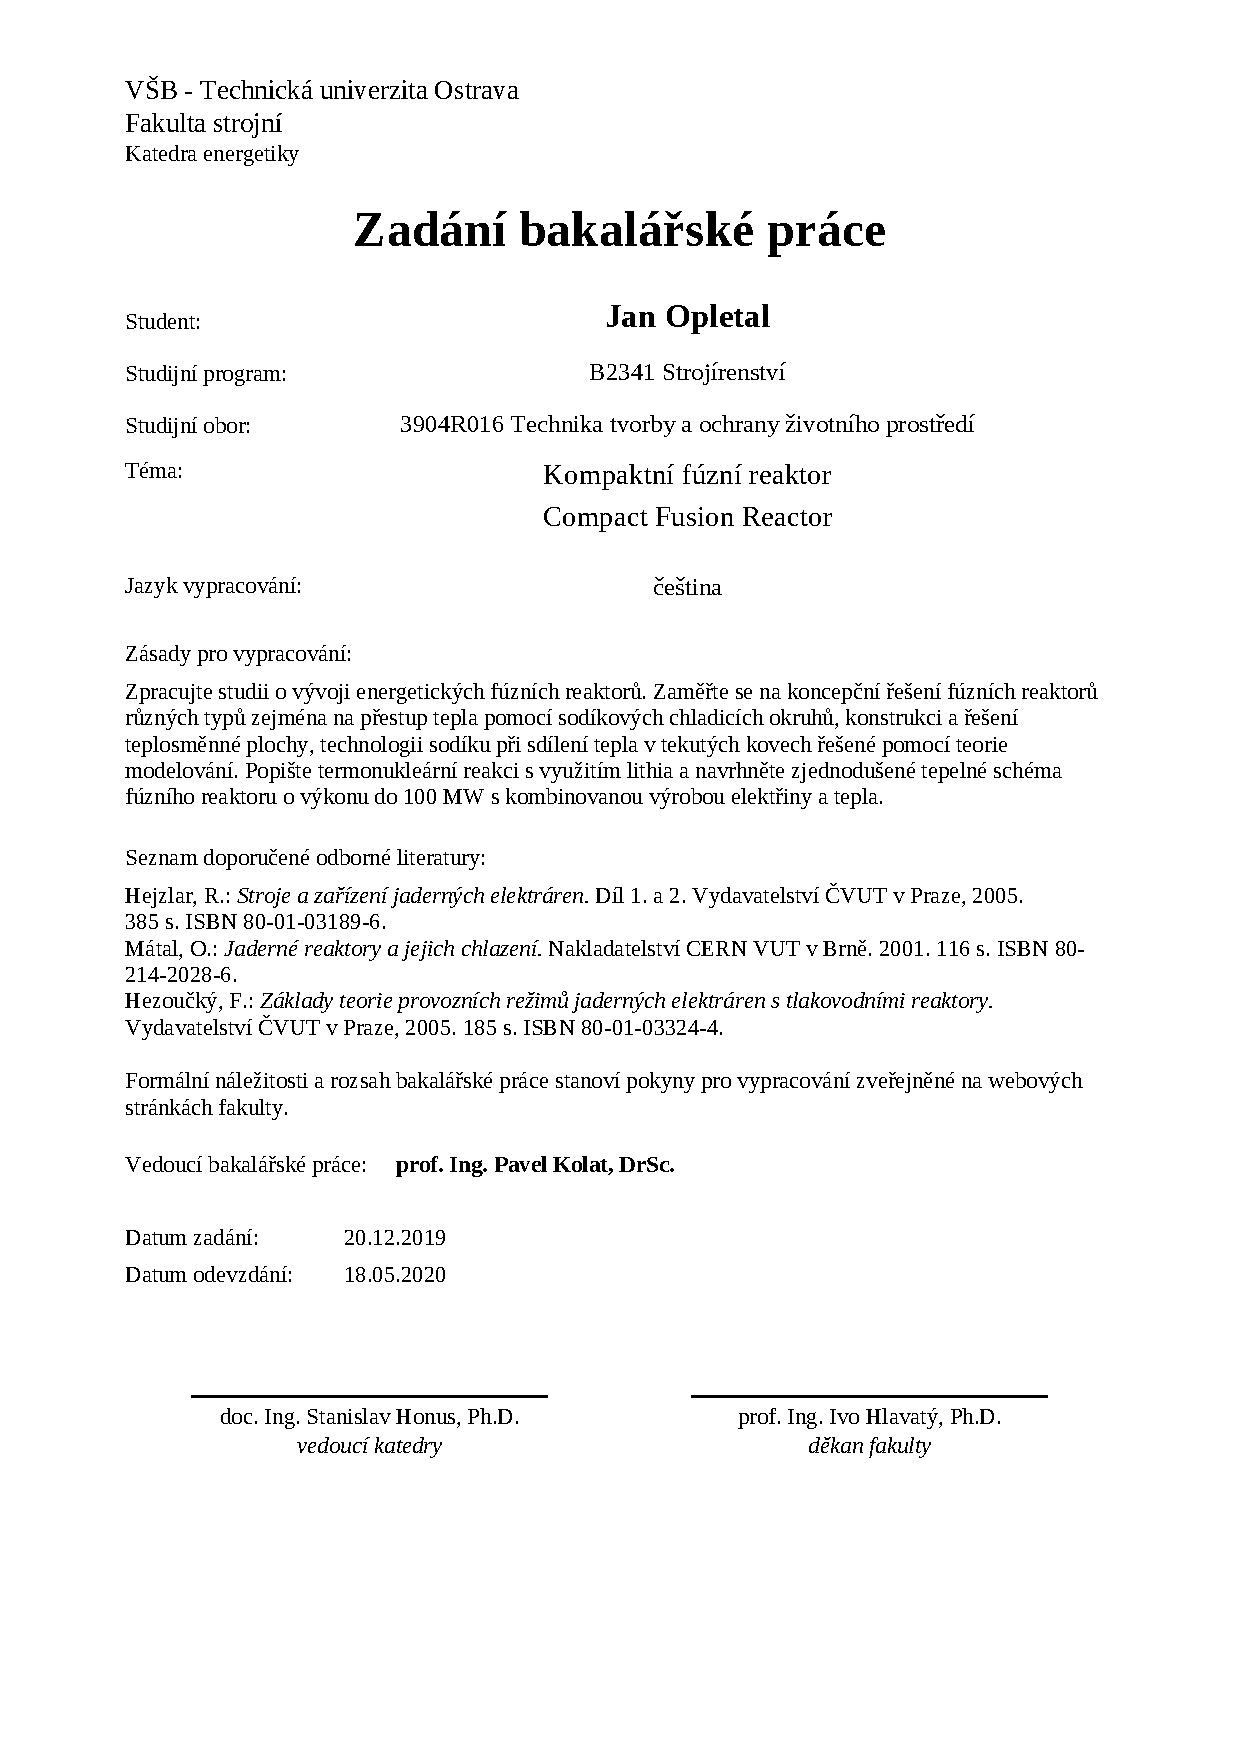
\includepdf[fitpaper=true, pages={1}]{config/assignment.pdf}

%%%% declaration/annotation
\subfileinclude{chapters/declaration_annotation}

%%%% TOC
\tableofcontents

%%%% nomenclature using \msym \msho commands
\subfileinclude{chapters/nomenclature}

\setcounter{page}{1}   % sets counting pages from start
\pagenumbering{arabic} % arabic numbering

%%%% introduction
\subfileinclude{chapters/introduction}

% head/footnote settings for chapters
\pagestyle{fancy}	
\fancyhf{}
\rhead{Diplomová práce}
\lhead{VŠB -- TUO}
\chead{your name}
\lfoot{Title name}
\rfoot{\thepage}
\renewcommand{\headrulewidth}{1pt}
\renewcommand{\footrulewidth}{1pt}


%%%% chapters
\subfileinclude{chapters/chapter_01}

\subfileinclude{chapters/chapter_02}

\subfileinclude{chapters/chapter_03}

\subfileinclude{chapters/chapter_04}

\subfileinclude{chapters/chapter_05}

\subfileinclude{chapters/chapter_06}

\subfileinclude{chapters/chapter_07}

\pagestyle{plain} 

%%%% conclusion
\subfileinclude{chapters/conclusion}

%%%% bibliography
\addcontentsline{toc}{section}{Seznam použité literatury}
\bibliographystyle{config/czechisounsrt}
\bibliography{main}

%%%% appendixes/thanks
\subfileinclude{chapters/appendix}	
		
\end{document}


